\chapter{\label{chap:spelunky}Spelunky}
Spelunky\footnote{http://www.spelunkyworld.com/original.html} é um jogo onde o
jogador incorpora um aventureiro que decide explorar uma caverna misteriosa. O
local contém tesouros, mas também está repleto de perigos. O objetivo principal
do jogador é explorar estas cavernas subterrâneas e coletar a maior quantia de
tesouros possível enquanto evita ser abatido pelos diversos inimigos e
armadilhas espalhadas pelo ambiente. A Figura \ref{fig:spelunky-gameplay}
ilustra uma partida do jogo.

\begin{figure}[htb!]
\centering
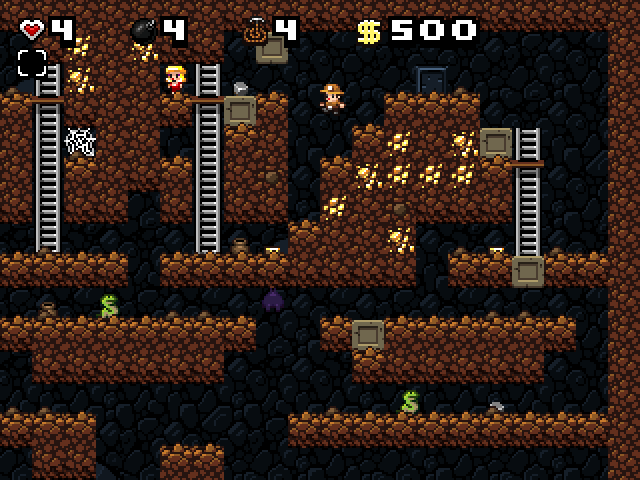
\includegraphics[width=.65\textwidth]{fig/spelunky-pc-screen.png}
\caption{\label{fig:spelunky-gameplay}Exemplo de partida de spelunky, mostrando
elementos do jogo como o jogador, a caverna, os inimigos, os tesouros, entre
outros.}
\end{figure}

O jogo se enquadra no gênero \textit{platformer}, estilo de jogo que envolve
guiar um personagem através de plataformas suspensas e obstáculos para obter
progresso no jogo. Também faz uso de alguns dos elementos-chave do gênero
\textit{roguelike} -- tipo de jogos que se popularizou na década de 80
caracterizados por sua dificuldade, enfoque em exploração de ambientes e
narrativa fantasiosa --, como \textbf{geração procedural} e \textbf{morte
permanente}. Os níveis de Spelunky são gerados proceduralmente, ou seja, utiliza
um algoritmo capaz de gerar automáticamente os elementos que irão compor o
nível. Isto significa que não existe uma maneira de se memorizar estratégias
específicas de um mapa em Spelunky, pois ao início de cada partida o mapa é
gerado de maneira única e os tesouros, itens e obstáculos são dispostos de
maneira diferente, fazendo com que o jogador tenha que aprender a lidar com os
elementos do jogo de forma individual, combinar este conhecimento e estabelecer
uma estratégia para vencer seus obstáculos e ser bem sucedido. A seção
\ref{section:spelunky-procgen} explica em maiores detalhes o algoritmo utilizado
para geração procedural. Além disso, o jogo conta com o conceito de morte
permanente, que faz com que o jogador, ao ter seus pontos de vida esgotados,
tenha que recomeçar o jogo desde seu início, perdendo todo o progresso obtido
até então.


%----------
\section{\label{section:spelunky-goals}Objetivos}
Apesar de o \textbf{objetivo principal} em Spelunky ser completar todos os
níveis, o jogo baseia a qualidade das partidas utilizando um sistema de
\textit{high scores}. Para tal, faz uso de uma série de métricas para
classificar os jogadores ao término de uma partida. Estas métricas são:

\begin{itemize}
	\item \textbf{Pontuação:} Mede a quantidade de tesouros obtidos pelo jogador
	no decorrer da partida. Existem diversos tipos de tesouros, como barras de
	ouro, pedras preciosas e estatuetas sagradas. Salvas as estatuetas sagradas,
	que devem ser carregadas até o fim do nível, o jogador precisa simplesmente
	tocar um tesouro para coletá-lo. Os tesouros se encontram espalhados pelo
	chão, dentro do terreno, dentro de baús ou são deixados por certos inimigos
	ao serem abatidos.

	\item \textbf{Tempo:} Mede o tempo para completar a partida. Começa a contar
	a partir do momento em que o jogador entra no primeiro nível e para de
	contar no fim do último nível. A contagem de tempo é interrompida durante as
	transições de nível e quando o jogador pausa a partida.

	\item \textbf{Abates:} Quantidade de inimigos abatidos pelo jogador durante
	a partida. Mortes acidentais de inimigos -- cair de um penhasco, acionar uma
	armadilha, etc. -- não aumentam este contador.

	\item \textbf{Salvamentos:} Quantidade de donzelas em perigo que foram
	resgatadas pelo jogador. Geralmente existe uma donzela em perigo por nível,
	mas existe a possibilidade -- mesmo que pequena -- de uma donzela não
	aparecer em alguns níveis. Para resgatar uma donzela, o jogador deve
	carregá-la com vida até a saída do nível.
\end{itemize}

Embora o jogo ofereça 4 métricas de classificação diferentes, a comunidade de
jogadores de Spelunky não mostra interesse significativo em atingir quantidades
elevadas de número de abates e número de salvamentos, se concentrando apenas em
atingir pontuações máximas e em concluir o jogo no menor tempo
possível\footnote{Comunidade de ranking de jogadores de Spelunky:
https://mosstier.com}. Pode-se concluir, portanto, que os \textbf{objetivos
secundários} mais importantes são a pontuação final e o tempo de partida. A
Figura \ref{fig:spelunky-scores} mostra um exemplo de pontuação final obtida.

\begin{figure}[htb!]
\centering
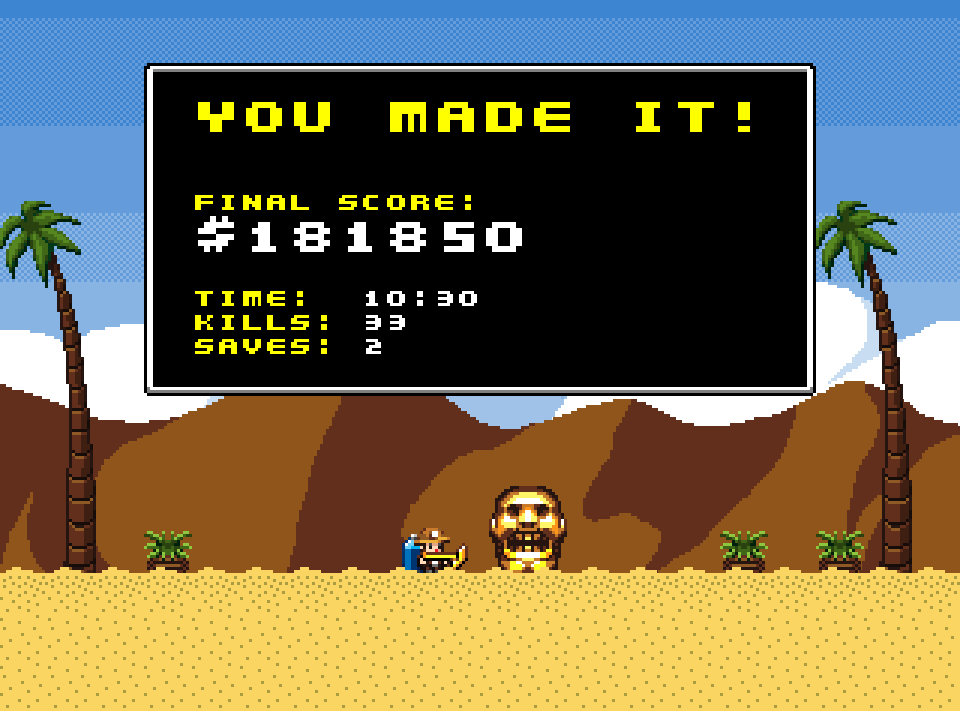
\includegraphics[width=.65\textwidth]{fig/spelunky-score.png}
\caption{\label{fig:spelunky-scores}Exemplo de pontuação final obtida ao fim de
uma partida de Spelunky.}
\end{figure}


%----------
\section{\label{section:spelunky-structure}Estrutura do jogo}
Uma partida de Spelunky é dividida em \textbf{níveis}, cada um sendo
representado por um mapa diferente. O jogador, ao entrar em um nível, é
posicionado na parte superior do mapa. Como não é informado ao jogador a posição
exata da saída, ele deve explorar o ambiente até encontrá-la. A saída sempre
está localizada em algum lugar na parte mais inferior do mapa. Ao utilizar a
saída, o jogador é enviado para o próximo nível e não pode retornar ao mapa que
acabou de completar.

O jogo é dividido em 4 \textbf{áreas} principais: \textbf{As Minas} (níveis 1 a
4), \textbf{A Selva} (níveis 5 a 8), \textbf{As Cavernas de Gelo} (níveis 9 a
12) e \textbf{O Templo} (níveis 13 a 16). Cada área possui um estilo de mapa e
aparência única. A dificuldade do jogo também aumenta gradativamente conforme o
jogador avança pelas áreas, principalmente porque os inimigos vão se tornando
cada vez mais fortes. O último nível do Templo é o \textbf{Covil de Olmec}. onde
o jogador deve enfrentar e derrotar \textbf{Olmec}. Após derrotar o inimigo
final, o explorador é recompensado com uma estatueta gigante feita de ouro e o
jogo termina.


\subsection{Atalhos}
É possível, ao iniciar uma partida, burlar este progresso entre áreas e ir
diretamente para as três ultimas áreas do jogo utilizando atalhos, criados pelo
personagem conhecido como \textbf{Homem do Túnel}. Para ter acesso a estes
atalhos, o jogador deve primeiramente auxiliar o Homem do Túnel a criá-los. O
personagem sempre aparece ao fim do último nível das primeiras três áreas do
jogo, se oferecendo para criar uma passagem secreta que leva ao início da área
que o jogador está prestes a chegar. Para criar a passagem, o jogador deve ceder
três vezes -- em partidas separadas -- ao Homem do Túnel uma mistura de tesouros
e itens.

Uma vez construídas, estas passagens são permanentes e podem ser acessadas ao
início de uma partida. Contudo, é importante ressaltar que, ao burlar etapas do
jogo, a pontuação do jogador não será contada para os \textit{high scores}.


\subsection{Áreas Secretas}
Além das áreas principais, existem duas áreas secretas: \textbf{O Mercado Negro}
e \textbf{A Cidade de Ouro}. Estas áreas do jogo são fundamentais para se obter
equipamentos e grandes quantidadeds de tesouros, mas o jogador só obterá acesso
a elas se respeitar uma série de requisitos impostos pelo jogo.

Para entrar no Mercado Negro, o jogador deve encontrar sua entrada -- que estará
oculta dentro do terreno do mapa -- enquanto explora a área da selva. O jogador
pode utilizar um item especial chamado \textbf{Udjat Eye} para ajudá-lo a
encontrar a entrada da área. O uso do item não é necessário, mas é aconselhável,
pois é quase impossível de localizar a entrada sem ele. Dentro do mercado negro,
o jogador encontrará vários comerciantes e terá a oportunidade de trocar seus
tesouros por equipamentos e itens diversos.

Entrar na Cidade de Ouro é muito mais complexo e é considerado um dos maiores
desafios do jogo, pois requer que o jogador colete uma série de artefatos
egípcios e execute uma longa cadeia de ações ao longo da partida. A Cidade de
Ouro é idêntica a um nível do Templo, mas o terreno é feito de ouro maciço --
podendo ser destruído com bombas -- e contém muito mais tesouros para coletar.
Além disso, o nível contém uma estátua dourada gigante feita de ouro e pedras
preciosas que pode ser destruída pelo jogador. As etapas para entrar na Cidade
de Ouro são:

\begin{enumerate}
	\item Coletar o \textbf{Udjat Eye}: O primeiro artefato se encontra dentro
	de um baú em algum nível da primeira área do jogo, as Minas. O jogador deve
	localizar a chave deste baú -- que se encontra no mesmo nível -- para poder
	abrí-lo. O Udjat Eye é capaz de encontrar a localização exata da entrada do
	Mercado Negro. O artefato pisca e brilha quanto mais próximo da entrada o
	jogador estiver, facilitando a localização da entrada.

	\item Coletar o \textbf{Ankh}: O segundo artefato se encontra no Mercado
	Negro e pode ser comprado (ou furtado) de um comerciante específico que
	vende somente este ítem. O Ankh oferece ao jogador uma segunda vida, caso
	venha a sucumbir.

	\item Coletar o \textbf{Hedjet}: O terceiro artefato pode ser obtido nas
	Cavernas de Gelo. Para obtê-lo, o jogador deve localizar um Moai\footnote{
	Estrutura monolítica com aparência humana. Os Moai foram esculpidos pelos
	Rapa Nui, habitantes nativos da Ilha de Páscoa.} e se morrer próximo a ele.
	O Ankh trará o jogador de volta a vida dentro do Moai e permitirá que o
	jogador colete o Hedjet.

	\item Coletar o \textbf{Cetro}: O quarto e último artefato podde ser obtido
	na última área do jogo, o Templo. O jogador deve encontrar e derrotar a
	Múmia, um dos inimigos mais fortes do jogo. Ao morrer, a múmia deixará o
	Cetro no chão. O Cetro é diferente dos outros itens porque, na verdade, é
	uma arma. Ele solta raios laser de cor rosa em formato de anel que perseguem
	e matam o inimigo mais próximo.

	\item Localizar a \textbf{Porta Dourada}: A última etapa do processo é
	encontrar a entrada da Cidade de Ouro, localizada em algum dos níveis do
	Templo. O jogador deve abandonar o Cetro e utilizá-lo como chave na Porta
	Dourada.
\end{enumerate}

Não é necessário que o jogador acesse as duas áreas secretas do jogo, mas as
quatro áreas principais devem necessáriamente ser visitadas, a não ser que o
jogador utilize um atalho. A Figura \ref{fig:spelunky-run} ilustra a relação
entre as áreas e o progresso de uma partida de Spelunky.

\begin{figure}[htb!]
\centering
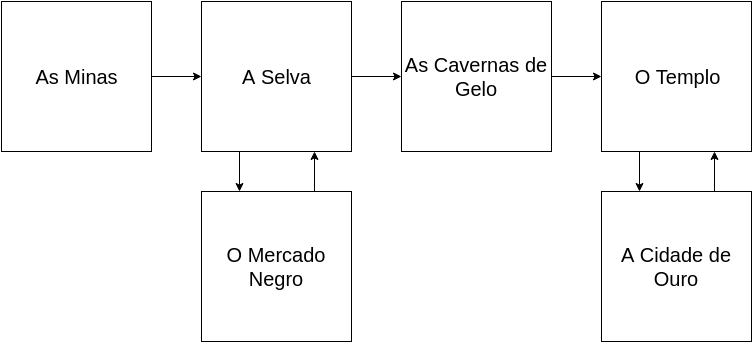
\includegraphics[width=.65\textwidth]{fig/spelunky-run.png}
\caption{\label{fig:spelunky-run}Relação entre as áreas de Spelunky durante uma
partida do jogo.}
\end{figure}


%----------
\section{\label{section:spelunky-controls}Controle do Personagem}
Os controles básicos em Spelunky são relativamente simples. Para se deslocar
pelo mapa, o jogador pode enviar comandos ao personagem para \textbf{caminhar},
\textbf{correr} e \textbf{pular}. O explorador também pode se \textbf{pendurar}
com as mãos na lateral de uma plataforma e subir e descer escadas. Como a
visibilidade do mapa é limitada a tela, o jogador pode \textbf{mover a câmera}
levemente na vertical ao \textbf{olhar para cima} ou se \textbf{agaixar},
aumentando sua visibilidade do ambiente. O explorador pode \textbf{utilizar
bombas e cordas} para auxiliar no deslocamento pelo nível. As bombas causam uma
explosão que elimina os inimigos e também desobstrui passagens. Já as cordas
permitem que o personagem atinja partes do mapa que não seriam acessíveis ao
pular, por estarem muito elevadas. Existe a possibilidade, também, de
\textbf{comprar itens} e \textbf{realizar apostas} com tesouros nas lojas dos
comerciantes.

A complexidade nos controles de Spelunky surge com a combinação de ações com
objetos, acessórios e equipamentos. O jogador pode \textbf{carregar um
item} em suas mãos e utilizá-lo quando desejar. O efeito depende do item
equipado atualmente. Por exemplo, se estiver carregando uma pedra, ele o
arremessará para longe. Se estiver segurando uma espingarda, ele realizará um
disparo. Os acessórios e equipamentos também modificam o funcionamento de ações.
Alguns acessórios podem fazer com que o personagem pule mais alto ou seja capaz
de se agarrar nas paredes. Portanto, é necessária atenção para os itens
coletados e equipados atualmente pelo explorador.


%----------
\section{\label{section:spelunky-procgen}Algoritmo de Geração Procedural de
Níveis}
% entrar em detalhes


%----------
\section{\label{section:spelunky-obstacles}Obstáculos}
% inimigos (listar)
% armadilhas (listar)
% ambiente (quedas, lava, etc.)


%----------
\section{\label{section:spelunky-items}Itens}
% três categorias diferentes: consumíveis, acessórios e armas
% listar todos e dar breve explicação


%----------
\section{\label{section:spelunky-dev}Desenvolvimento e Distribuição}
O jogo foi desenvolvido por Derek Yu -- utilizando o motor de desenvolvimento de
jogos \textit{GameMaker} (Versão 8.0 Pro) -- e lançado gratuitamente para a
plataforma \textit{Windows} em dezembro de
2008\footnote{https://forums.tigsource.com/index.php?topic=4017}. No fim de
2009, o criador optou por liberar o código fonte do jogo, permitindo sua
distribuição não-comercial e
modificação\footnote{http://www.spelunkyworld.com/files/COPYING.txt}. A
liberação do código fonte de Spelunky pode ser considerada um marco muito
importante, pois permitiu que fossem criadas modificações para o jogo. Estas
modificações, que podem ser encontradas no fórum oficial da
\textit{Mossmouth}\footnote{http://mossmouth.com/forums/index.php} -- empresa
desenvolvedora de jogos criada por Derek Yu --, são correções de \textit{bugs},
mapas customizados ou até mesmo modos de jogo completamente diferentes do jogo
original. Pode-se dizer que dar esta liberdade para a comunidade do jogo é um
dos fatores que ajuda a manter sua base de jogadores e atraem novos jogadores
até hoje.

O motor GameMaker disponibiliza diversas ferramentas que facilitam o trabalho
do desenvolvedor. Contando com funcionalidades como editores de
\textit{scripts}\footnote{Código desenvolvido para o controle dos
comportamentos dos elementos do jogo.} e de \textit{sprites}\footnote{Elementos
visuais do jogo, tais como o personagem, o fundo, os inimigos. Representados
como uma ou mais imagens, permitindo que as mesmas sejam animadas.},
gerenciadores de eventos, entre
outras\footnote{http://sandbox.yoyogames.com/downloads/docs/gmaker80.pdf}, o
GameMaker oferece um ótimo suporte ao desenvolvedor para a criação de jogos. O
motor disponibiliza uma linguagem de programação própria para seus
\textit{scripts}, a \textit{GameMaker Language}, ou \textit{GML}.
